\documentclass{article}

%%%% 
%%%% try also class: {IEEEtran}
%%%%

\usepackage{graphicx}
\input list
\lstset{language=C,style=demostyle}

\begin{document}
\title{STC \LaTeX\ demo}
\author{Victor Eijkhout}
\date{2021}
\maketitle

\section{An introduction to \LaTeX}

In 1978 Donald Knuth started working \TeX, 
which is pronounced `tek' or `Tau Epsilon Chi',
and that really doesn't stand for anything.

Then in the mid-80s, Leslie Lamport
wrote an extension to \TeX, called \LaTeX.

Observations:
\begin{enumerate}
    \item Input lines do not correspond to output lines
    \item A blank line makes a new paragraph.
    \item A backslash introduces a command.
\end{enumerate}
We will prove interesting stuff in
section~\ref{sec:math}.

\section{Math}
\label{sec:math}

\TeX was written for very math-y books.
\[ \int_0^\infty xdx=\infty \]
Formulas can also be $\int x=1/2x^2$ in text.
Formulas can also be numbered:
\begin{equation}
\int_0^\infty xdx=\infty
\label{formula:inf}
\end{equation}
Combining formula~\ref{formula:inf} and stuff
gives stuff.

\begin{figure}[ht]
    \centering
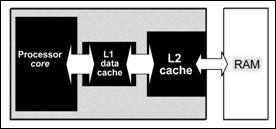
\includegraphics[scale=1.1]{graphics/caches}
    \caption{Caption}
    \label{fig:my_label}
\end{figure}

%\lstverbatiminput{sourcefile} ?
\begin{lstlisting}
int x=5;
for (int i=0; i<n; i++)
 y = x*x;
\end{lstlisting}
Earlier results were proved in \cite{AdJo:colorblind}.

\bibliographystyle{plain}
\bibliography{math}
\end{document}

